% 2010 年江西卷文科第 20 题：两个共边正三角形 BCD、MCD 与垂线段 AB。
% 来源 PDF：普通高考/2010/2010江西文.pdf，SHA-256 c8c86a7272df02211069e27098dcaf04a5cd8af9a9b4d54ffd14a8eb91347af3。
% 原页：第 2 页（A3 三栏）第 1 栏中部，书页码 610。
% 重绘依据：△BCD 在底面，△MCD 与底面垂直并向上折起；AB⊥平面 BCD，AB=2√3；
%   AM、CM、DM 为实线，BM、BD 在遮挡处按原页保留实线，BC 与 MD 用虚线。
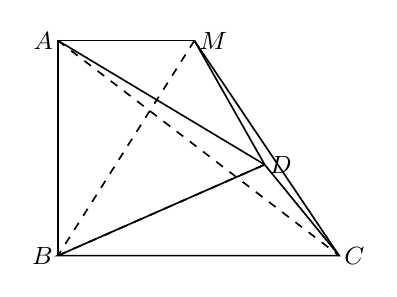
\begin{tikzpicture}[semithick, scale=1.05, every node/.style={inner sep=1.6pt, font=\small}]
  \coordinate (B) at (0,0);
  \coordinate (C) at (3.4,0);
  \coordinate (D) at (2.5,1.1);
  \coordinate (A) at (0,2.6);
  \coordinate (M) at (1.65,2.6);

  \draw (B) -- (C) -- (D) -- cycle;
  \draw (B) -- (A) -- (M);
  \draw (M) -- (C);
  \draw (M) -- (D);
  \draw (A) -- (D);
  \draw[dashed] (A) -- (C);
  \draw[dashed] (B) -- (D);
  \draw[dashed] (M) -- (B);

  \node[left] at (A) {$A$};
  \node[left] at (B) {$B$};
  \node[right] at (C) {$C$};
  \node[right] at (D) {$D$};
  \node[right] at (M) {$M$};
\end{tikzpicture}
